% !TEX root = ../Ausarbeitung.tex
\section{Einleitung}
\label{sec:Einleitung}

Bis kurz vor der Jahrtausendwende führte die Virtualisierung von Servern ein Schattendasein und jeder Service wurde auf einem dedizierten Server zur Verfügung gestellt. Dabei war es keine Seltenheit, dass Server sehr gering ausgelastet waren, da der laufende Service nicht die gesamte Leistung der Hardware benötigte und der Ausfall eines nicht redundanten Servers einen Totalausfall eines Services bedeutete. Eine Beispielhafte dedizierte Serverkonstellation stellt folgende Grafik dar:
\begin{figure}[H]
	\begin{center}
		
\includegraphics[width=1\textwidth]{vm1.png}
	\end{center}
	\caption[Serverauslastung ohne Virtualisierung]{Serverauslastung ohne Virtualisierung \footnotemark}
	\label{fig:HW1}
\end{figure}
\quellefoot{1}{https://www.redhat.com/cms/managed-files/server-usage-500x131.png}
\newpage
Um diese und weitere Probleme zu lösen, gewann die Virtualisierung von Servern zum Anfang des neuen Jahrtausends immer mehr an Bedeutung und ist heutzutage ein fester Bestandteil vieler großer Unternehmen. Dabei werden auf einem physikalischen System mehrere Dienste zusammengefasst, die sonst nur einen Bruchteil der Leistung benötigen würden. Dadurch kommen noch andere Vorteile wie z.B. das Erstellen von Snapshots und das dynamische Verschieben der virtuellen Maschinen zum tragen die folgende Grafik zeigt die Auslastung der virtualisieren Server:
\begin{figure}[H]
	\begin{center}
		
\includegraphics[width=1\textwidth]{vm2.png}
	\end{center}
	\caption[Serverauslastung mit Virtualisierung]{Serverauslastung mit Virtualisierung \footnotemark}
	\label{fig:HW1}
\end{figure}
\quellefoot{2}{https://www.redhat.com/cms/managed-files/server-usage-for-virtualization-500x131.png}
\newpage
Doch auch die Virtualisierung von Servern birgt noch verbesserbare Nachteile. So entsteht durch das Betriebssystem der virtuellen Maschinen ein deutlicher Overhead, da diese zur Laufzeit etliche Services benötigen. Durch die virtualisierten Betriebssysteme wird die Hardware deutlich mehr beansprucht und die Startzeit ist relativ lange. Somit war die IT-Welt nicht in der Lage, wozu die Menschheit längst in der Lage ist: Güter in Container verpacken und diese Container aufgrund dem Standardisierten Format auf den verschiedensten Verkehrswegen zu transportieren. Um diese Lösung in die IT zu portieren, wurden auch hierfür sogenannte Software-Container entwickelt.
Software-Container setzen wie die Schiffscontainer an dem Punkt Portabilität an. Es soll nicht für jeden Service ein zusätzliches Betriebssystem virtualisiert werden, sondern der Container soll nur das zusätzlich beinhalten was er für den Service benötigt und trotzdem isoliert von den anderen Container auf der Hardware laufen. Außerdem soll es wie bei den virtuellen Maschinen möglich sein, dynamisch Ressourcen zuzuweisen.\cite{12005068320161201,redhat} Die folgenden Grafik verdeutlicht nochmals den eingesparten Overhead bei Containern verglichen mit virtuellen Maschinen: 
\begin{figure}[H]
	\begin{center}
		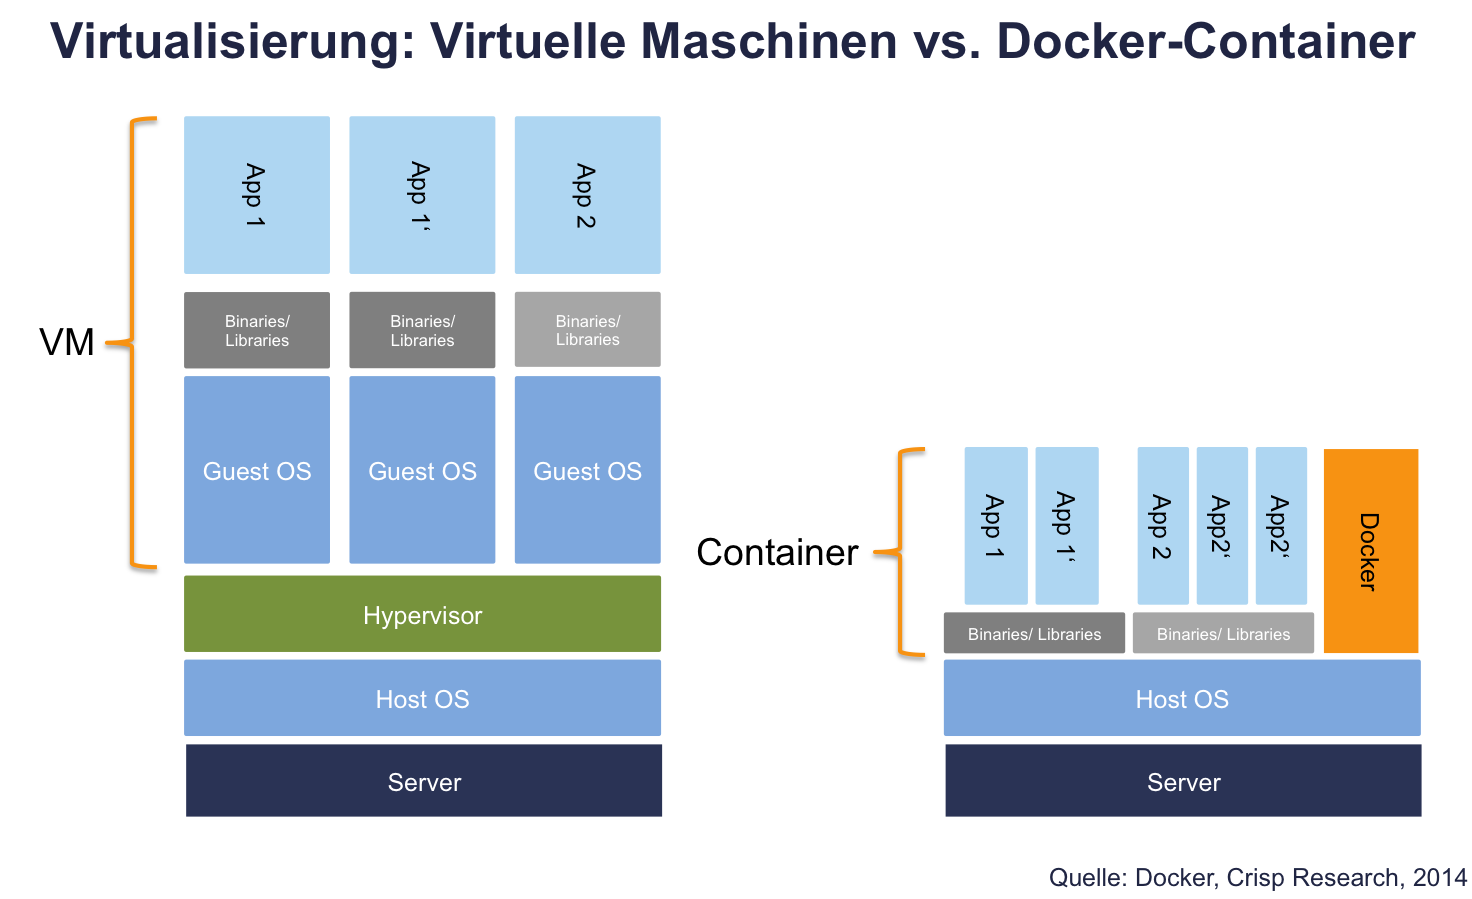
\includegraphics[width=1\textwidth]{containerundvm.png}
	\end{center}
	\caption[Vergleich Container und VM]{Vergleich Container und VM \footnotemark}
	\label{fig:HW1}
\end{figure}
\quellefoot{3}{https://images.computerwoche.de/bdb/2668601/738x415_f5f5f5.jpg}



